\documentclass{article}

\usepackage[english]{babel}
%\usepackage[utf8x]{inputenc}
\usepackage{amsmath}
\usepackage{graphicx}
%\usepackage[colorinlistoftodos]{todonotes}

\title{Consistency, Accuracy, Valence and Topology in Constraint Satisfaction Models of Attitudes: Comment on Dalege 2016}
%\shorttitle{Formalization of the CAN Attitude Network Model}
%\author{Mark G. Orr, Emily N. Stark, David C. Plaut}
%\affiliation{Biocomplexity Institute at Virginia Tech}

%\abstract{Your abstract here.}

\begin{document}
\maketitle

\section{Introduction}
Over the past 2 decades, the social psychological literature has successfully co-opted computational modeling approaches from cognitive science to address a range of phenomena:  causal attribution, stereotype, attitude formation, impression formation, and personality (REFs READ BOOK, new and old; Van Overwalle book; Holyoak and others; Eliot Smith).  Constraint satisfaction, typically formalized as an artificial neural network, holds a singular place in social psychology because it not only fits historical and existing theoretical notions across a range of phenomena (REF see Simon \& Holyoak, 2002) but also has provided novel mechanistic insights into said phenomena (REF see READ 1998 introduction). (Hereafter CS will be used interchangeably with constraint satisfaction.) The properties and characteristic behaviors of artificial neural networks using constraint satisfaction are well understood under the condition that the underlying network (graph) typology and the activation functions of the nodes are bounded withing common parameterizations (e.g., a fully recurrent neural network with sigmoid units) (REF PDP, HOPFIELD, ETC.). This knowledge has served the social psychological research community well, as there are several off-the-shelf platforms for implementing well-understood constraint satisfaction models.

The study of attitude formation and change serves as a prototypical example of what constraint satisfaction offers in a theoretical sense.  First, it represents the notion of cognitive consistency when presented with a attitude object.  Second, when attitudes are conceptualized as an associative memory system, the degree of error in reproducing a set of learned examples captures the notion of accuracy in forming an attitude with respect to the accumulation of past experiences with an attitude object. (The notion of attitude as a memory process falls in-line with a more traditional conceptualization of what the attitude construct means (e.g., Eagly and Chaiken, 1993).) Third, constraint satisfaction integrates accuracy and consistency with a high degree of parsimony. Learning to accurately represent the attitude object generates long-term, stable constraints on the limit-points of the system while, at the same time,  the shorter-term, immediate context/input constraints the same limit-point.  Simply put, the limit-point of the system at any moment depends on both the weights (from learning) and the input (immediate context).  The last point is the most prominent precisely because it suggests that the distinction between accuracy and consistency is a convenience of labeling:  constraints are satisfied and whether these come from the weights or from the input is irrelevant.  It is true, however, that the metrics for consistency and accuracy reflect different aspects of a constraint satisfaction system--the former as energy/goodness and the latter as error.

A central aspect of attitudes that is not directly captured in constraint satisfaction models is the valence of the components that comprise the system (e.g., the set of features associated with the attitude object).  In practice, this means that the valence of the nodes in a CS neural network serve only as labels for interpretation of the behavior of the system and play no role in the learning process or the computational machinery of satisfying constraints.  We will clarify this notion by example using a well-known visual illusion: the Necker cube.  The Necker cube is a simple line-drawing for which the visual impression, for many viewers, is a rapid switch in orientation from left-facing to right-facing, with some degree of stability once each orientation is fixated.  Rumelhart, et al (REF PDP V2 Chap 14) developed a CS model of the Necker cube visual illusion that illustrates our point. The weights in the Rumelhart model, although hand-wired and fixed, can be conceptualized for our purposes as the accumulation of past experience via a learning process.  The model has 16 nodes so that each vertex of the cube is represented twice.  When the model is presented with input, it usually settles into one of two limit points, each of which reflects the past experience and the current inputs of the model.  The interpretation of the limit-points is straight-forward because the nodes of the neural network are clearly labeled with respect to their interpretation (each vertex is associated with either the left- or right-facing cube).  The interpretation is, to our point, completely external to the CS process.  Simply put, the system doesn't care about the meaning of its nodes or whether the limit-point is supposed to be interpreted as left- or right-facing.  It cares about parallel satisfaction of the constraints.  

Existing CS models of attitude formation use two approaches that are a variation of the Necker cube.  First, a subset (or all) of the units are designated a prioi as representing positive or negative valence (ORR/Plaut, OrrThrushPlaut, van Overwalle, Ehret). Second, units are valenced by their activation level, and the activation level is designated as representing positive or negative valence (Monroe/Read, Spellman). In either case, valence is formally outside of the constraint satisfaction system.   \footnote{Another approach to attitude formation was put forth by Eiser and colleagues REFS using a feed-forward pattern associator with contingent feedback (creating a kind of reinforcement learning).  Valence was still determined by the researcher, but during the training/feedback cycle.} 

Whether or not theoretical gap is not quite clear. However we cannot stress enough the importance of this subtle theoretical point.  

Recently, in this journal, Dalege et al posited a new conceptualization of attitude formation and change that incorporates both constraint satisfaction and the 

that distinguished learning (generating a network over time) and on-the-fly processing (attitude formation given an attitude object) with respect to the role that valence played.  Specifically, the generation/learning of an attitude over time, by the CAN model,  is hypothesized to incorporate the valence of nodes in a network while the formation of an attitude given a stimulus (internal or external) did not consider valence whatsoever (e.g., a node in the network might represent an attribute of the attitude object or a belief about the attitude object).  

Importantly, the dichotomy in terms of the respective role of valence drives the system towards a particular network topology, a small-world topology, which is hypothesized, by Dalege et al, to afford a reduction in energy *e.g., Hopfield, or an increase in goodness (e.g., Rumelhart and McClelland); roughly, the stability of the attitude.  In short, a sparsely connected but clustered network topology (small-world REF Watts \& Strogats) may play a role in the constraint satisfaction process in relation to attitude formation and change.   In particular:  quote Dalege " ".  

Although the Dalege et al paper provided a seemingly unique and novel theoretical contribution to computational social psychology in general and to attitudes in particular, it was, unfortunately, presented sans historical context.  Network topology, in general, and its relation to the performance of artificial neural networks (e.g., accuracy, capacity, speed, retrieval) has been under study for the past 20 years. Of particular interest here is the role of small-world topology, which saw much study in the early 2000s, just after its discovery (of the small-world).  The quintessential example is a paper by Bohland \& Minai, (REF 2001) in which it is demonstrated via simulation that associative memory performance is dependent on topology, worst with regular ring-lattice and best with random.  But small-world was pretty darn good. This is daming for the accuracy hypothesis...for Dalege. It was hypothesized that the small-world topology, althoguht much closer to a regular lattice than a fully random network in terms of its rewiring probability.  In short, the small-worlds neural network literature captures well the objectives of why topology might matter.  To Summarize. Some key domains: creativity, image/pattern completion, associative memory, network growth and learning, neuro-anatomy?  Some key objective functions: accuracy of learning, storage capacity, speed of learning?, pattern-retrival, etc.  Some key topologies:  neurally constrainted, sparse, etc.   

What is interesting about the CAN model is that the model criterion is the energy at the networks limit-points (stable states) (See Hopfield, 1982, for a historical exploration of this).  So, effectively, small-world topology is supposed to produce less energy, everything else equal. Quote Dalege "To deal with this trade-off between optimization of consistency and accuracy, attitude networks are proposed to show clustering (i.e., differnt sets of evaluative reactions are hightly interconnected.  Clustering allows for energy reduction wihtin clusters (e.g., all evaluative reactions toward a person that pertain to the dimension of warmth are highly aligned) but also allows for accuracy by having unalighned or even misalighned clusters that do not cost much energy...[p 6 para 4]" 

However, despite the interesting theoretical development offered by the CAN model, the evaluation of the principal claim, that small-world topology reduces limit-point energy is difficult, given the evidence marshaled by Dalege et al.  Specifically, the empirical evidence provided is cross-sectional (aggregate) analysis of the correlatsions among a set of beliefs, when estimated using a specialized statistical appraoch, show that in fact the structure of an attitude network is in fact small world.  However, this evidence implies nothing about the processing characteristics and how the small world affect them. The actual processing was not explored. However, in lieu of exploration of the information processing dynamics of the CAN attitude model topology, Dalege et al offered a set of rudimentary simulations that calculated the energy (using the Ising Hamiltonian function) in three node attitude networks that showed that energy .  The small-world, their central claim, was not addressed even peripherally.  To summarize, the empirical work relied on a specific parameterization of a statistical modeling approach, which was, to our knowledge and testing not discussed here.  The small-world phenomena was not tested in the rudimentary simulations.  It is therefore difficult to assess the claims of the CAN attitude model w.r.t the relation between limit-point energy and small-world network topology.

The present work does not address the generative mechanism directly, but simply tests the degree to which the expected network topology from the hypothesized generative mechanism (a small-world) has any effect on the energy of limit-points in the system.    To do this 

The fundamental assumptions of the CAN attitude model are: 1) the dynamics are an attractor neural network (for them it is an Ising model) in which each node represent single evaluative reactions to an attitude object, 2) the system optimizes for consistency w.r.t. the valence of the nodes; that is, nodes of the same valence should have excitatory connections between them as well as the logical compliment, 3) the system attempts to also represent accuracy w.r.t. to the relation between the attitude object and the evaluative reaction; that is, nodes of differing valence may have excitatory connections between then as well as the logical compliment, and 4) the topology of the attractor neural network will be small-world.

Algorithmically, consistency in the sense put forth by the CAN model above arises from two independent mechanisms. One is the dynamics of the recurrent networks in terms of its limit-cycle when activated in any way (this type of consistency is strictly the same constraint satisfaction algorithm used in many models of social cognition).  The other mechanism represent how the CAN model generates the network that represents an attitude in its totality.  In essence, the former captures the short-term, immediate activation of the attitude and the latter captures long-term learning over time.

An important subtlety in this system is that the valence of the evaluative beliefs is only incorporated into the learning mechanism and is not represented in the constraint satisfaction algorithm.  This theoretical duality is coupled with the notion that the topology of attitude networks are small-world.  The driving idea is that a small-world, such that within clusters are like valenced evaluative reactions with excitatory connections and between clusters are opposite valenced evaluative reactions with inhibitory clusters, buys a reduction in energy in the Ising model across limit points.  By the CAN model it is not clear whether the constraint on learning to include valence generates small-world or whether the 




Recently, in this journal, the notion of constraint satisfaction as a mechanism representing attitude formation and change was given an additional theoretic commitment coming directly from network science:  sparsely connected but clustered network topology may play a role in the constraint satisfaction process.   In particular:  quote Dalege " ".

This is a non-trivial hypothesis for which the 

In this present article, we explore directly the processing characteristics within a constraint satisfaction framework as a funciton of the degree to which the network topology is a small world. Specifically, through a set of simulations, we parametrically vary the control parameter in the original small world generating mechanism (probability of rewiring) to define a set of weights.  These weights then served as connection weights in a fully recurrent artificial neural network (RNN).  The RNN provided the basis for a set of simulations in which the degree of energy (goodness) at simulation end was the primary dependent variable.  To be clear, the approach developed here takes a deductive small-world approach such that under some p, G implies SM as opposed to the empirical inductive approach used by Dalege et al. 

\section{The CAN Attitude Model Small-World Argument}
\label{sec:sim}
Central to the CAN model is the notion that attitude formation dynamics (in its immediate, on-the-fly sense) are governed by Ising dynamics, a probabilistic account of constraint satisfaction models in certain physical systems.  \footnote{We will not explore further that Dalege did not make reference to the important role that Ising-like models influenced artificial neural networks in the early 1980s, a point that embed the CAN model in the larger picture of parallel constraint satisfaction models in psychology because it links the CAN model direclty to the general PDP approach}.  Suffice it to say that the Ising model is a constraint satisfaction model that inherently deals with accuracy and consistency given accuracy defined as mismatch between input and output and and consistency defined by a measure of goodness or energy (e.g., Hopfield, 1982).  In short, parallel constraint satisfaction, in the 

LETS DO AN EXAMPLE GRAPHIC OF THE SMALL WORLD IDEA....

A critical departure from the standard parallel constraint satisfaction story is the additional assumption that attitude networks will have similar valences (positivitiy or negativity).  Its probably true that this assumption makes sense in the 'real-world.'  











\section{Methods}

\subsection{Weight Generation}
In order to achieve a small world network, we will begin with a lattice network and rewire edges with a set probability, $p_{rewire}$. As $p_{rewire}$ increases, we will see more defined clusters due to the shortcuts "across" the ring". As these shortcuts are created, clusters will emerge due to the decreased degree of the node from which the rewired edge originated. For an illustration of how the network changes across $p_{rewire}$ see Figures \ref{fig:p0}, \ref{fig:p25}, \ref{fig:p50}, \ref{fig:p75}, \ref{fig:p100}
\\
In order to correctly weight the rewired graph, we used the following weight formula:

\[ W(i,j) =    \left\{
\begin{array}{ll}
      w_{ij}'' = 1 & \exists \text{ } m,n \text{ such that } w_{ij}' = w_{mn} \\
      w_{ij}'' = -1 & \text{otherwise} \\
\end{array} 
\right. \]
 Where $w_{ij}$ are the original weights, $w_{ij}'$ are the weights immediately following the rewire, and $w_{ij}''$ are the final weights. This process was carried out using the distance matrix before and after the rewires to determine the shortcuts created due to rewiring. For a more detailed algorithm, see the appendix.




\subsection{Simulations}
MO

\subsection{Analysis}
After the simulations finish and the networks stable out, their Goodness is recorded. Our results are given for a graph of size $n = 100$ but is consistent with larger values for $n$ as well. There were 10 values for the number of initial neighbors, $k$, ranging from 9 to 49. These values were chosen based on the restriction $$ln(n) << k << n$$ from WATTS CITE HERE. Additionally, 10 values of $p_{rewire}$ were tested ranging from 0 to 1. There were 10 trials, $i$, per treatment where the ring was rewired once per trial. This resulted in 1000 total values for Goodness. We plotted both the raw Goodness as well as Goodness normalized across the values of $k$ as seen in Figures \ref{fig:G}  and \ref{fig:Gnorm}. 

\begin{figure}
\centering
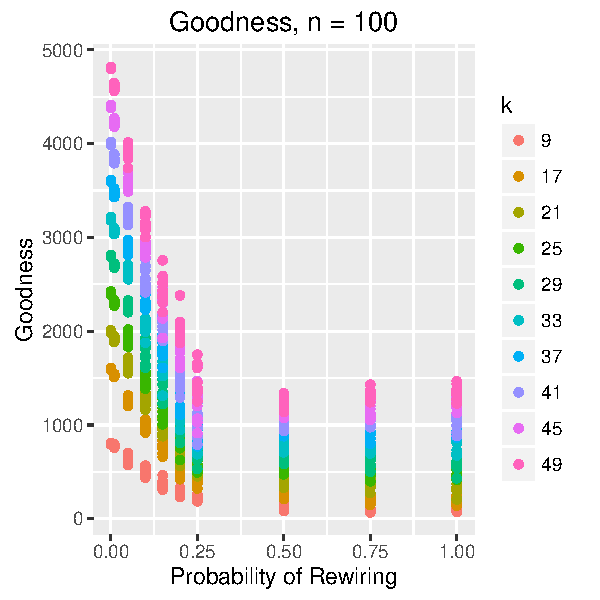
\includegraphics[width=1\textwidth]{1-G_n100.pdf}
\caption{\label{fig:G}Goodness for a size $n = 100$ Graph}
\end{figure}

\begin{figure}
\centering
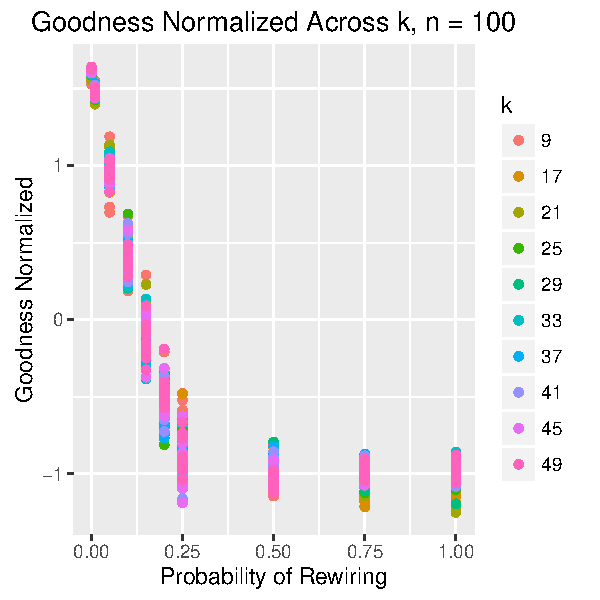
\includegraphics[width=1\textwidth]{2-G_norm_n100.pdf}
\caption{\label{fig:Gnorm}Normalized Goodness for a size $n = 100$ Graph}
\end{figure}


 To get another look at the data, we also plotted the mean Goodness per treatment (defined as unique combinations of $k$ and $p_{rewire}$) as well as the standard deviations. In order to get a sense of normality we also calculated the level of skewness (rudimentarily defined as the difference between the mean and the median) and ran Anderson-Darling tests on treatments. It is important to note that with 100 treatments, we would expect to see $0.05(100)=5$ cases of type I error, which is consistent with our findings. These results are depicted in Figures \ref{fig:Gmean} through \ref{fig:Gskew}.

\begin{figure}
\centering
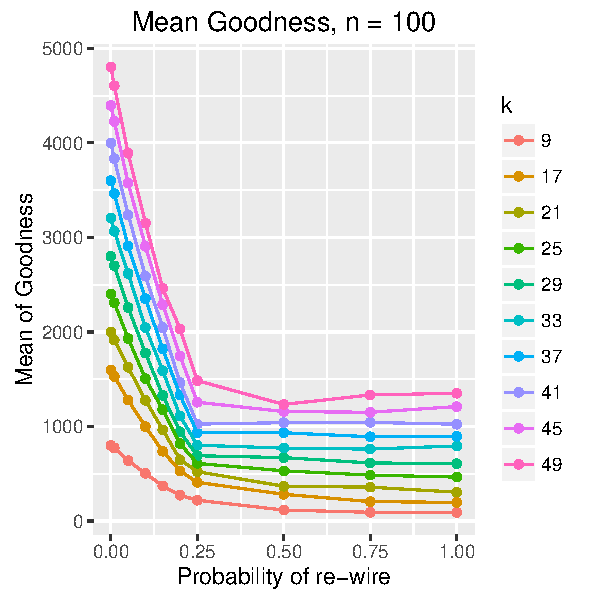
\includegraphics[width=1\textwidth]{3-meanG_by_p_k_n100.pdf}
\caption{\label{fig:Gmean}Mean Goodness per treatment for a size $n = 100$ Graph}
\end{figure}

\begin{figure}
\centering
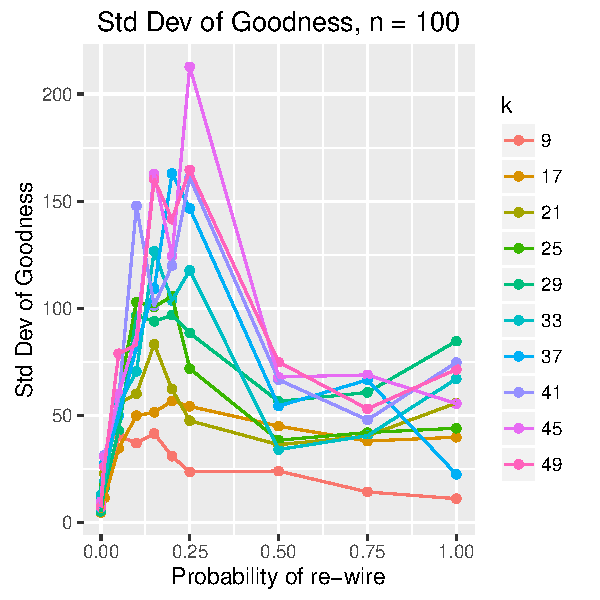
\includegraphics[width=1\textwidth]{4-sdG_by_p_k_n100.pdf}
\caption{\label{fig:Gsd}Standard Deviation of Goodness per treatment for a size $n = 100$ Graph}
\end{figure}

\begin{figure}
\centering
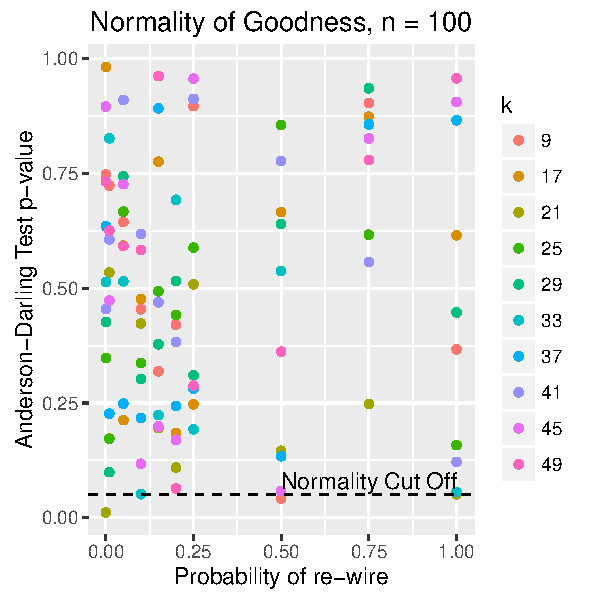
\includegraphics[width=1\textwidth]{5-normG_by_p_k_n100.pdf}
\caption{\label{fig:Gad}p-values for Anderson-Darling test of Goodness by treatments for a size $n = 100$ Graph. The dashed line represents the $\alpha = 0.05$ significance level.}
\end{figure}

\begin{figure}
\centering
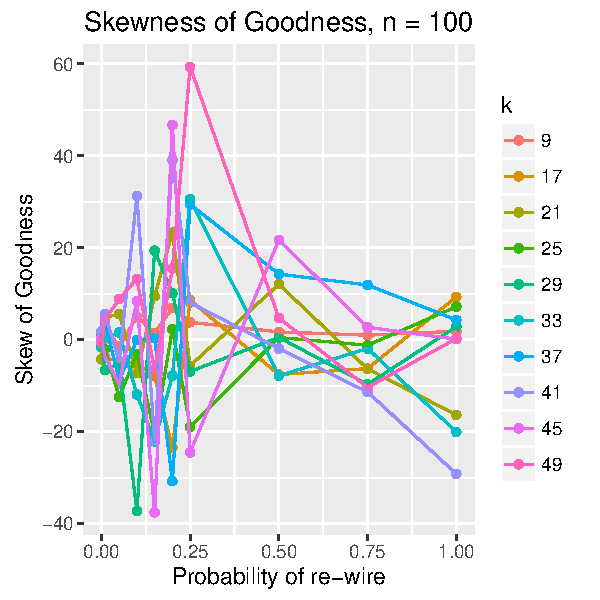
\includegraphics[width=1\textwidth]{6-skewG_by_p_k_n100.pdf}
\caption{\label{fig:Gskew}Skewness of Goodness by treatment, defined as $mean-median$ for $n = 100$ Graph}
\end{figure}

\section{Results}
Goodness is positively correlated with the graph's clustering coefficient ($r^2 = 0.7197$) and weakly, negatively correlated with the graph's the average characteristic path length ($r^2 = 0.2095$). Additionally, the Goodness is strongly correlated with the interaction of the two ($r^2 = 0.8226$). A scatter plot showing this can be found in figure \ref{fig:ccg}

\begin{figure}
\centering
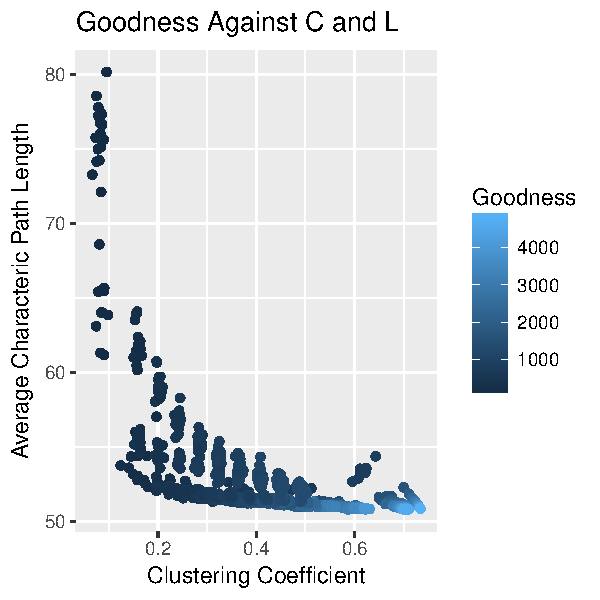
\includegraphics[width=1\textwidth]{8-cpl_vs_clus_G_col.pdf}
\caption{\label{fig:ccg}Average characteristic path length plotted versus clustering coefficient colored to represent goodness}
\end{figure}


It was also found that goodness is weakly, negatively correlated with the probability or rewiring and weakly, positively correlated with the number of initial neighbors a node has ($r^2 = 0.3293$, and $r^2 = 0.3556$). While a linear model with both parameters and the interaction, results in an adjusted $r^2$ value of 0.7265. This is represented in figure \ref{fig:pkg}

\begin{figure}
\centering
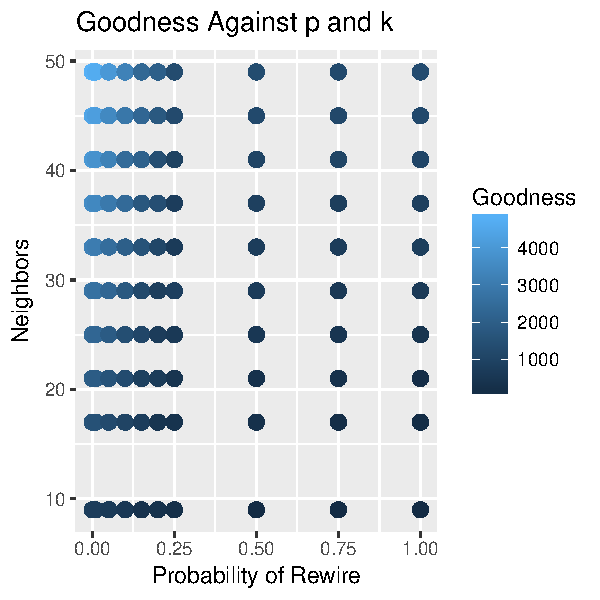
\includegraphics[width=1\textwidth]{7-k_vs_p_G_col.pdf}
\caption{\label{fig:pkg}Initial neighbors plotted versus the probability of rewiring colored to represent goodness}
\end{figure}



\section{Discussion:  What have we learned and who cares?}
\label{sec:disc}
What about the glaring omission of Hopfield?  "...recently proposed application of the Ising model (Ising, 1925) to psychological data (Eps....2014). The ising model belings to the class of Markov Random Fidel models used in network analysis and constitutes the Markov Random Field for binary data (Kindermann ...1980).  Originating in statistical physics, the Ising model has been applied in several research areas.  The interested reader is referred to Epskamp et al (in press) for a thorough discussion of the Ising model." pg 5 para 3. AND "To summarize, the Ising model represents a promising conceptualization of attitudes as this conceptualization readily integrates both interactions between evaluative reactions and the need to maximize cognitive consistency...: pg 6, para 2.  WE MIGHT use this to argue that the these folks are coming from a different conceptual area of psychology, one that does not think clearly in terms of information processing as it is realted to cognitive science or theoretical neuroscience.  COULD THIS be used in the intro to make their case even weaker?


\section{Appendix}
\subsection{Weight Generation}
In order to identify which edges are the rewired edges we used the distance metric in the package iGraph. It is seen in Figure \ref{fig:p100} that some original edges remained even though there was a 100\% probability of edge rewire. This is not surprising, as some rewired edges will be rewired to a position where an edge already exists. Because of this, we cannot simply count all rewired edges as between-cluster edges, or some original edges may be labeled incorrectly.
\\
In order to correctly identify between-cluster and within-cluster edges, we use the distance function in the iGraph package. We are able to output an $n \times n $ matrix which reports the length of the shortest path between any two nodes. It is useful to consider the case with no rewirings, Figure \ref{fig:p0}, to think about clusters. In this case, there are as many clusters as nodes that are not mutually exclusive. Considering the case with $n = 14$ and starting with two neighbors, we see two clusters identified in Figure \ref{fig:p0n14c}. In this case a cluster can be thought of as a collection of nodes in which the shortest distance between any two nodes in a given cluster is 1. 
%THINK ABOUT THIS AND GET BACK TO ME...DISTANCE = 1? HELPFUL TO THINK ABOUT STOCHASTIC/STATE DIAGRAMS AND CLASSES OF CLUSTERS.
\\
If an edge is reassigned to a position where there was previously no edge, then the distance between the nodes which contain the new edge will have gone from a quantity greater than one to one. In this way, a new edge can be considered a "short cut", which is consistent with the existing literature on small-world networks (see ...). In order to efficiently capture this and thus assign a negative weight to any between-cluster edge and a positive weight to all within-cluster edges, we can simply take the difference of the distance matrix before and after rewiring. If the distance decreased, we reassign that value to be $-1$ and any distance that stayed the same or increased we assign a 1 in order to preserve any pre-existing edges. It should be noted that we are only using $\pm 1$ in the difference matrix because we are not concerned with the magnitude of the weights, but simply the sign. This method will result in a matrix that has a non-zero entry for every element. In order to delete all the non-existent edges in the rewired graph, we simply have to multiple element-wise the rewired weight matrix with the new difference matrix. This will create negative weights anywhere there is a short cut (i.e. between-cluster edge) and positive edges elsewhere. This process is shown in steps in Figure \ref{fig:wt_gen_steps}.




\begin{figure}
\centering
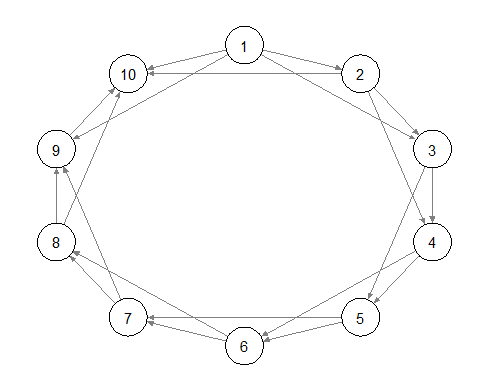
\includegraphics[width=1\textwidth]{p0.png}
\caption{\label{fig:p0}$p_{rewire}=0$}
\end{figure}

\begin{figure}
\centering
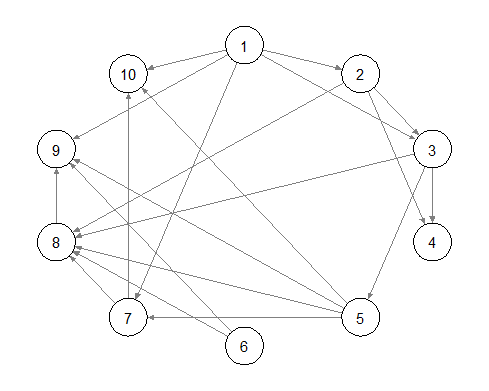
\includegraphics[width=1\textwidth]{p25.png}
\caption{\label{fig:p25}$p_{rewire}=.25$}
\end{figure}

\begin{figure}
\centering
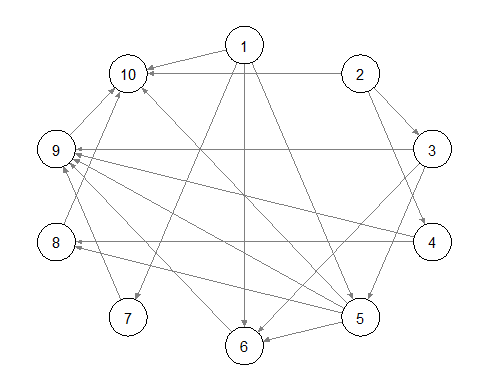
\includegraphics[width=1\textwidth]{p50.png}
\caption{\label{fig:p50}$p_{rewire}=0.50$}
\end{figure}

\begin{figure}
\centering
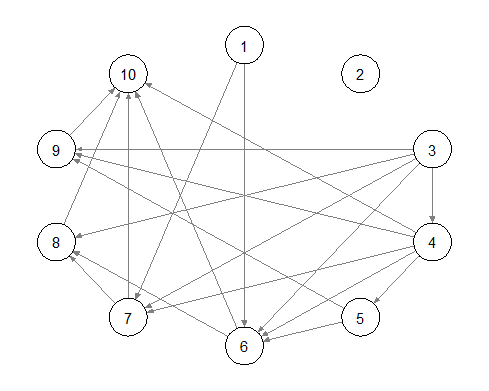
\includegraphics[width=1\textwidth]{p75.png}
\caption{\label{fig:p75}$p_{rewire}=0.75$}
\end{figure}

\begin{figure}
\centering
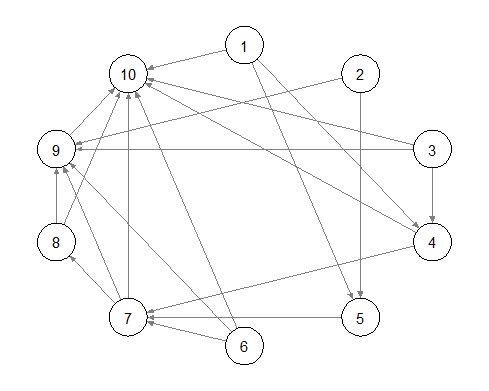
\includegraphics[width=1\textwidth]{p100.png}
\caption{\label{fig:p100}$p_{rewire}=1$}
\end{figure}

\begin{figure}
\centering
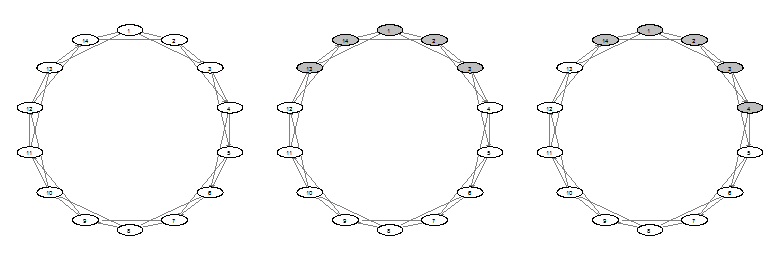
\includegraphics[width=1\textwidth]{p0n14c.png}
\caption{\label{fig:p0n14c}Ring graph with $n = 14$, $k = 2$ as well as two identified clusters.}
\end{figure}

\begin{figure}
\centering
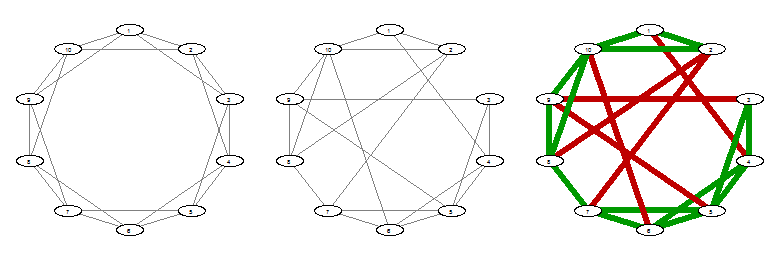
\includegraphics[width=1\textwidth]{wt_gen_steps.png}
\caption{\label{fig:wt_gen_steps}Beginning with $n=10, k=2, p_{rewire}=0.25$, we see the initial ring, the rewiring, and the weight assignments.}
\end{figure}

In order to better understand how the parameters $p_{rewire}$ and $k$ affected the structure of the graph, we looked at the average clustering coefficient and the average characteristic path length of all combinations of the parameters. It is shown in figure \ref{fig:clus_cpl} that as $k$ increases, clustering increases and characteristic path length decreases, and as $p_{rewire}$ increases, clustering experiences a sharp decrease and then levels out while characteristic path length dips and then increases, with a more dramatic rise the lower that $k$ is.

\begin{figure}
\centering
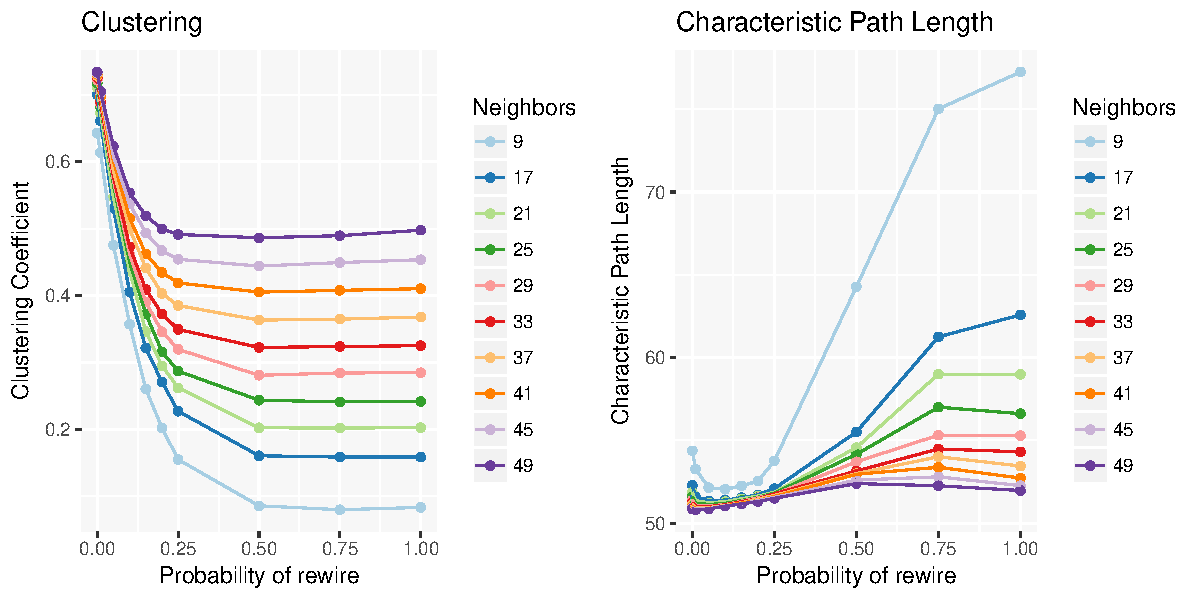
\includegraphics[width=1\textwidth]{metrics_plots.pdf}
\caption{\label{fig:clus_cpl}Average network metrics on size $n=100$ graphs}
\end{figure}


\bibliography{example}


\end{document}